% Provenance (never printed): cycle 4 SVT, "La planete Terre, l'environnement":
% glaciers and their landforms, the cryosphere, the glaciations told; see
% sources/book1/PROVENANCE.md. Book 1, grade 8, chapter 5.
% Vocabulary guard: owns glacier; ice sheet + ice shelf + iceberg (one
% definition); sea ice; permafrost; U-shaped valley + moraine (one
% definition); ice age. "Glacial period", "interglacial" and "glacial cycle"
% belong to Book 2 g12 past-climates: here "the ice ages and the warmer times
% between them", in prose. Albedo belongs to Book 2 g10: here "reflects".
% Buoyancy and water expanding as it freezes are physics: recalled in prose.
\chapter{地球上的冰}\label{ch:g8:ice-on-earth}

下面两张照片于同一地点拍摄，地点是阿拉斯加的一处泻湖，
两张照片相隔 26 年。1990 年，一条宽阔的冰舌沿着\omterm{def:g1:landscapes-around-us:landform}{山谷}一直延伸到水边。
2016 年，\omterm{def:g8:ice-on-earth:glacier}{冰川}已向\omterm{def:g1:landscapes-around-us:landform}{山谷}上游退缩，变得更窄；
原先\omterm{def:g8:ice-on-earth:glacier}{冰川}让出的空间，已被树木和裸露的\omterm{def:g3:stones-pebbles-sand:rock}{岩石}覆盖。
卫星图像显示，1984 年至 2021 年间，佩德森\omterm{def:g8:ice-on-earth:glacier}{冰川}
的前缘后退了约 \qty{3.2}{km}。
% ledger: commons:pedersen, uw:pedersen

\begin{omfigure}
\begin{minipage}[t]{0.49\linewidth}\centering
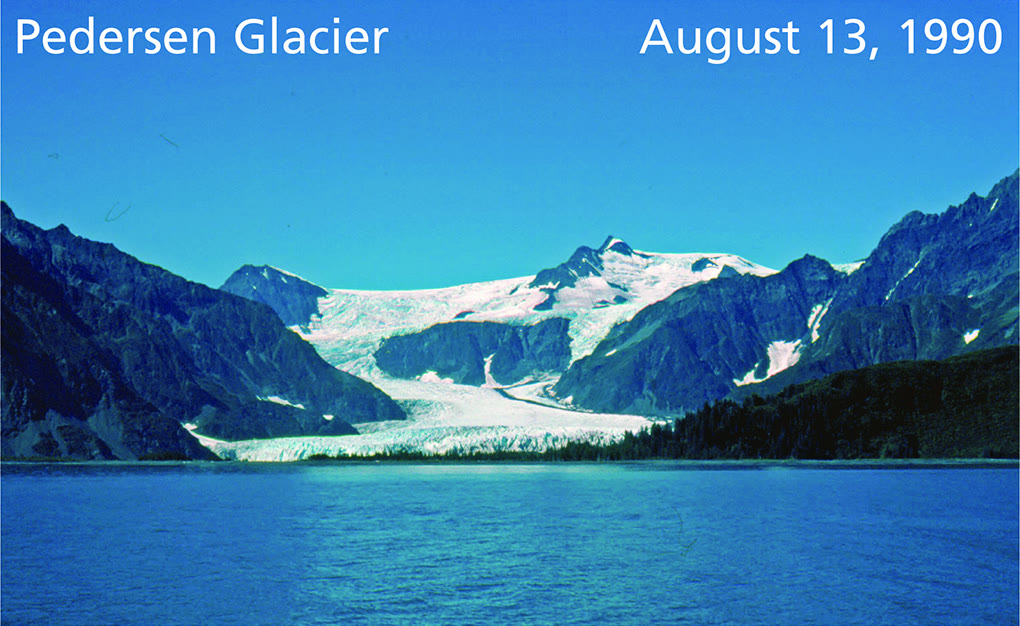
\includegraphics[width=\linewidth]{images/book1/g8-pedersen-1990.jpg}
\end{minipage}\hfill
\begin{minipage}[t]{0.49\linewidth}\centering
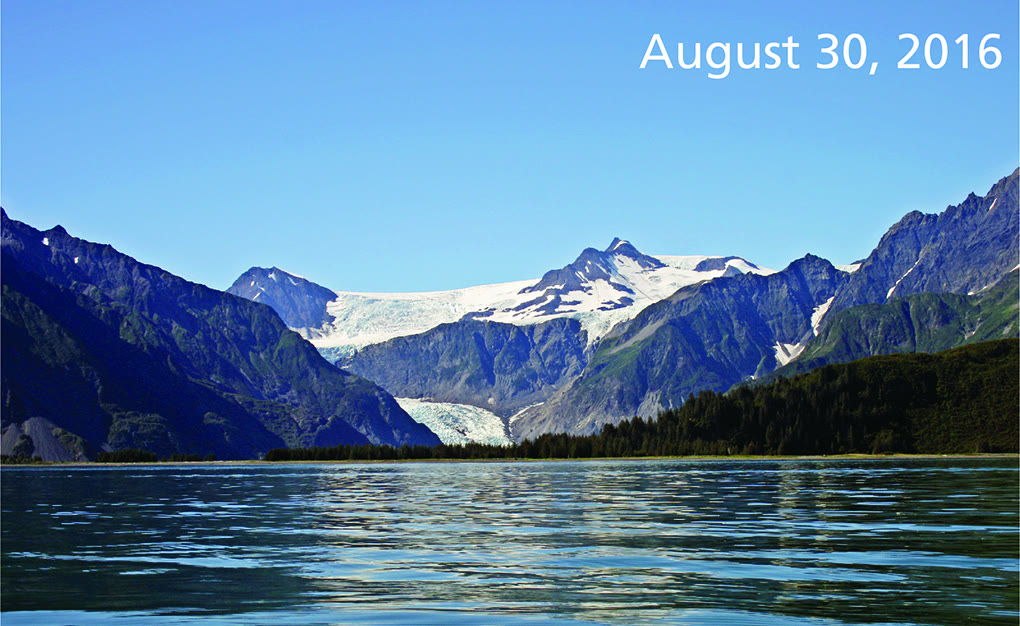
\includegraphics[width=\linewidth]{images/book1/g8-pedersen-2016.jpg}
\end{minipage}

\smallskip
{\small 佩德森\omterm{def:g8:ice-on-earth:glacier}{冰川}，阿拉斯加凯奈峡湾国家公园，
拍摄地点相同：左图为 1990 年 8 月 13 日（M.~Tetreau 摄），
右图为 2016 年 8 月 30 日（D.~Kurtz 摄）。美国国家公园管理局，
公有领域（经由维基共享资源）。}
% ledger: commons:pedersen
\label{fig:g8:ice-on-earth:pedersen}
\end{omfigure}

今天，冰覆盖着地球陆地面积的约十分之一。它分布在山地
\omterm{def:g1:landscapes-around-us:landform}{山谷}中，覆盖\omterm{def:g3:continents-and-oceans:poles}{南极}洲和格陵兰的两大\omterm{def:g8:ice-on-earth:ice-sheet}{冰盖}之上，位于极地
海域中，还隐藏于遥远北方的冻土之中。本章
将依次讨论这几处冰，以及冰如何塑造大地，
以及冰曾覆盖地球远大于今天范围的时期。
% ledger: nsidc:ice-cover

\begin{recall}
雪是\omterm{def:g4:clouds-rain-snow:precipitation}{降水}的一种：冰晶在云中生长，
未经融化便落下（见\cref{ch:g4:clouds-rain-snow}）。流水
\omterm{def:g5:water-shapes-the-land:erosion}{侵蚀}大地，搬运碎屑，并将其\omterm{def:g5:water-shapes-the-land:deposition}{沉积}在更下游的地方；
\omterm{def:g1:landscapes-around-us:water}{河流}切割出\omterm{def:g1:landscapes-around-us:landform}{山谷}（见\cref{ch:g5:water-shapes-the-land}）。海水
结冰时，盐分留在冰周围的水中
（见\cref{ch:g8:the-oceans}）。在物理学中，你已经学过：水结冰时体积膨胀，
因此冰的密度小于液态水，并且比它所排开的水轻的物体
会漂浮。
\end{recall}

\section{冰川}

在高山上，冬季降雪多于夏季融雪。
年复一年，新雪覆盖旧雪并将其压实。
雪晶彼此挤压在一起，其间的空气被挤出，
大约一年后，积雪变成\emph{粒雪}，
一种介于雪与冰之间的颗粒状物质。深埋越深，粒雪便变为坚硬的
固体冰；对大多数\omterm{def:g8:ice-on-earth:glacier}{冰川}而言，这一过程需要一百多年。
% ledger: nsidc:firn

\begin{definition}[冰川]\label{def:g8:ice-on-earth:glacier}
称\emph{冰川}\index{冰川}为一块冰体，由多年堆积的雪
在自身重力作用下，沿陆地表面缓慢向下坡移动。
\end{definition}
% ledger: nsidc:glacier-def

\omterm{def:g8:ice-on-earth:glacier}{冰川}分为两部分。在其上部，即\emph{积累区}，
每年降雪多于融雪，\omterm{def:g8:ice-on-earth:glacier}{冰川}得到冰量；在其下部，
即\emph{消融区}，每年融化的冰多于降雪，
\omterm{def:g8:ice-on-earth:glacier}{冰川}失去冰量。上部获得的冰不断向下流动，以补充
下部失去的冰。若两者保持平衡，\omterm{def:g8:ice-on-earth:glacier}{冰川}的前端，即其
\emph{冰舌末端}，位置保持不变。
% ledger: nsidc:glacier-zones

\begin{omfigure}
\begin{tikzpicture}[font=\footnotesize, >={Stealth[length=2mm]}, xscale=1.08]
  % bedrock
  \fill[black!13] (0,4.6) -- (2,3.9) -- (4,3.0) -- (6,2.0) -- (8,1.1)
    -- (10,0.45) -- (11,0.3) -- (13,0.15) -- (13,-0.5) -- (0,-0.5) -- cycle;
  % the ice body, two zones
  \begin{scope}
    \clip (0,5.5) -- (2,4.9) -- (4,4.0) -- (6,2.9) -- (8,1.8) -- (9.4,0.95)
      -- (10,0.45) -- (8,1.1) -- (6,2.0) -- (4,3.0) -- (2,3.9) -- (0,4.6) -- cycle;
    \fill[omIce] (0,-1) rectangle (5,6);
    \fill[omSea!85] (5,-1) rectangle (11,6);
  \end{scope}
  \draw[black!60] (0,5.5) -- (2,4.9) -- (4,4.0) -- (6,2.9) -- (8,1.8)
    -- (9.4,0.95) -- (10,0.45);
  \draw[black!70, line width=0.6pt] (0,4.6) -- (2,3.9) -- (4,3.0) -- (6,2.0)
    -- (8,1.1) -- (10,0.45) -- (11,0.3) -- (13,0.15);
  % snowline
  \draw[dashed, black!70] (5,2.5) -- (5,4.15);
  \node[anchor=south] at (5,4.15) {降雪量 = 融化量};
  % snowflakes and melting
  \foreach \x/\y in {0.5/6.1, 1.3/5.8, 2.1/5.5, 2.9/5.1, 3.7/4.8, 0.9/6.6, 1.7/6.3, 2.5/6.0, 3.3/5.6, 4.1/5.2}
    \node[omCold] at (\x,\y) {$\ast$};
  \foreach \x/\y in {6.4/2.8, 7.2/2.35, 8.0/1.9}
    \draw[omWarm, decorate, decoration={snake, amplitude=0.6mm, segment length=2mm}] (\x,\y) -- ++(0,0.6);
  % flow arrows inside the ice
  \draw[->, omDef, line width=0.9pt] (1.0,4.72) -- (2.2,4.30);
  \draw[->, omDef, line width=0.9pt] (3.0,3.95) -- (4.2,3.41);
  \draw[->, omDef, line width=0.9pt] (5.2,2.88) -- (6.4,2.28);
  \draw[->, omDef, line width=0.9pt] (7.2,1.84) -- (8.3,1.35);
  % moraine and meltwater
  \fill[omLithCongl] (10.15,0.42) .. controls (10.5,0.95) and (10.9,0.95) .. (11.2,0.29) -- cycle;
  \draw[omSea!60!black, line width=1.6pt] (10.05,0.38) .. controls (10.6,0.22) and (11.4,0.12) .. (12.9,0.08);
  % labels
  \node[align=center] at (1.9,7.15) {积累区：\\ 雪不断堆积，冰川获得冰量};
  \node[align=center] at (10.0,3.3) {消融区：\\ 冰融化，冰川失去冰量};
  \node[align=left, anchor=west, omDef] at (4.4,1.3) {冰体沿坡 \\ 向下流动};
  \draw[black!60] (10.0,0.5) -- (9.6,-0.1) node[below] {冰舌末端};
  \draw[black!60] (10.7,0.85) -- (11.3,1.4) node[above] {冰碛};
  \node[anchor=north east] at (12.9,0.0) {冰川融水溪};
  \node at (2.2,2.6) {基岩};
\end{tikzpicture}

{\small 从纵剖面看到的\omterm{def:g1:landscapes-around-us:landform}{山谷}\omterm{def:g8:ice-on-earth:glacier}{冰川}（示意图，未按比例绘制）。
虚线以上，降雪堆积的速度快于融化；虚线以下，
冰融化的速度快于降雪。冰体从一部分
流向另一部分。}
\label{fig:g8:ice-on-earth:long-section}
\end{omfigure}

固态的冰为何能够流动？\omterm{def:g8:ice-on-earth:glacier}{冰川}深处的冰在上方冰体的重压下，
会缓慢变形，就像一层厚厚的冷蜂蜜缓缓摊开。
\omterm{def:g8:ice-on-earth:glacier}{冰川}还会沿下方的\omterm{def:g3:stones-pebbles-sand:rock}{岩石}滑动，借助薄薄的水膜
或湿泥进行。\omterm{def:g8:ice-on-earth:glacier}{冰川}底部与\omterm{def:g3:stones-pebbles-sand:rock}{岩石}摩擦，其运动
比顶部更慢。大多数\omterm{def:g8:ice-on-earth:glacier}{冰川}缓慢而稳定地移动；少数\omterm{def:g8:ice-on-earth:glacier}{冰川}
会突然\emph{跃动}。1986 年，阿拉斯加的哈伯德\omterm{def:g8:ice-on-earth:glacier}{冰川}向前跃动，
每天前进约 \qty{10}{m}；有记录以来最快的跃动，发生在
1953 年巴基斯坦的库提亚\omterm{def:g8:ice-on-earth:glacier}{冰川}，其间三个月内平均每天前进约 \qty{112}{m}。
% ledger: nsidc:glacier-flow, nsidc:surges

当\omterm{def:g8:ice-on-earth:glacier}{冰川}在下方失去的冰量多于上方获得的冰量时，其冰舌末端
会向\omterm{def:g1:landscapes-around-us:landform}{山谷}上方后退，即\omterm{def:g8:ice-on-earth:glacier}{冰川}\emph{退缩}。退缩中的\omterm{def:g8:ice-on-earth:glacier}{冰川}
仍然沿坡向下流动，就像传送带一样；只是融化的速度快于流动的速度。
阿拉斯加的缪尔\omterm{def:g8:ice-on-earth:glacier}{冰川}在 1941 年充满了整个\omterm{def:g1:landscapes-around-us:landform}{山谷}，一直延伸到海边。
到 2004 年，其冰舌末端已后退 \qty{12}{km}，冰面
高度下降超过 \qty{800}{m}。
% ledger: nsidc:glacier-flow, nsidc:muir

\section{冰如何塑造山谷}

\omterm{def:g8:ice-on-earth:glacier}{冰川}是强大的\omterm{def:g5:water-shapes-the-land:erosion}{侵蚀}营力。冰体冻结在松散岩块上，
并将其拔起带走；冻结在\omterm{def:g8:ice-on-earth:glacier}{冰川}底部的石块像砂纸一样
刮擦下方的\omterm{def:g3:stones-pebbles-sand:rock}{岩石}。\omterm{def:g8:ice-on-earth:glacier}{冰川}将这些岩屑，从细粉
到巨石，像传送带一样沿\omterm{def:g1:landscapes-around-us:landform}{山谷}向下搬运，
并在冰融化处将其堆积下来。
% ledger: nps:u-valley

\begin{omfigure}
\begin{tikzpicture}[font=\footnotesize, >={Stealth[length=2mm]}]
  % V-shaped valley
  \fill[black!13] (0,3) -- (2.1,0.35) -- (2.5,0.35) -- (4.6,3) -- (4.6,-0.4) -- (0,-0.4) -- cycle;
  \draw[black!70, line width=0.6pt] (0,3) -- (2.1,0.35) -- (2.5,0.35) -- (4.6,3);
  \fill[omSea] (2.1,0.35) -- (2.5,0.35) -- (2.42,0.2) -- (2.18,0.2) -- cycle;
  \node[align=center] at (2.3,-0.85) {河流切出狭窄的 \\ V 形谷};
  % arrow
  \draw[->, line width=1pt] (5.0,1.5) -- (6.2,1.5) node[midway, above, align=center] {冰川 \\ 将其填满};
  % U-shaped valley
  \begin{scope}[xshift=6.6cm]
    \fill[black!13] (0,3) .. controls (0.6,1.0) and (0.9,0.25) .. (1.6,0.2)
      -- (3.0,0.2) .. controls (3.7,0.25) and (4.0,1.0) .. (4.6,3) -- (4.6,-0.4) -- (0,-0.4) -- cycle;
    \draw[black!70, line width=0.6pt] (0,3) .. controls (0.6,1.0) and (0.9,0.25) .. (1.6,0.2)
      -- (3.0,0.2) .. controls (3.7,0.25) and (4.0,1.0) .. (4.6,3);
    \draw[dashed, black!40] (0,3) -- (2.1,0.35) -- (2.5,0.35) -- (4.6,3);
    \draw[omCold, line width=0.9pt] (0.37,2.2) -- (4.23,2.2);
    \node[omCold, anchor=south, font=\scriptsize] at (2.3,2.2) {很久以前的冰面};
    \fill[omLithCongl] (0.75,0.95) .. controls (0.95,1.2) and (1.1,1.1) .. (1.2,0.6) -- cycle;
    \fill[omLithCongl] (3.85,0.95) .. controls (3.65,1.2) and (3.5,1.1) .. (3.4,0.6) -- cycle;
    \node[align=center] at (2.3,-0.85) {冰消失后：宽阔的 \\ U 形谷，两侧陡峭};
    \draw[black!60] (3.65,0.95) -- (4.85,0.6) node[right, align=left] {侧碛};
    \node[font=\scriptsize, black!55, align=center] at (2.3,1.6) {（虚线为原 V 形谷）};
  \end{scope}
\end{tikzpicture}

{\small 同一\omterm{def:g1:landscapes-around-us:landform}{山谷}在\omterm{def:g8:ice-on-earth:glacier}{冰川}作用前后的横剖面（示意图）。
\omterm{def:g8:ice-on-earth:glacier}{冰川}将狭窄的河谷刻蚀为宽阔的槽谷，
槽谷底部平坦、两侧陡峭，并沿槽谷两侧
留下岩屑堆积成的脊。}
\label{fig:g8:ice-on-earth:v-and-u}
\end{omfigure}

\begin{definition}[U 形谷与冰碛]\label{def:g8:ice-on-earth:glacial-landforms}
\emph{U 形谷}\index{U 形谷}是谷底宽阔平坦、两侧陡峭的\omterm{def:g1:landscapes-around-us:landform}{山谷}，
由\omterm{def:g8:ice-on-earth:glacier}{冰川}拓宽并加深原有的狭窄 V 形河谷而形成。
\emph{冰碛}\index{冰碛}是\omterm{def:g8:ice-on-earth:glacier}{冰川}遗留的岩屑堆积脊，岩屑大小从细粉
到巨石不等；沿\omterm{def:g1:landscapes-around-us:landform}{山谷}侧边分布的是\emph{侧碛}，
位于末端的是\emph{终碛}。
\end{definition}
% ledger: usgs:erratic, nps:u-valley, nps:moraines

\omterm{def:g8:ice-on-earth:glacial-landforms}{冰碛}是有用的线索。位于\omterm{def:g1:landscapes-around-us:landform}{山谷}远端、附近没有冰体的终碛，
表明\omterm{def:g8:ice-on-earth:glacier}{冰川}曾经延伸到的最远位置；\omterm{def:g1:landscapes-around-us:landform}{山谷}坡上位置较高的侧碛，
则表明\omterm{def:g8:ice-on-earth:glacier}{冰川}曾经有多厚。一块
孤立地搁在原野上的巨石，其\omterm{def:g3:stones-pebbles-sand:rock}{岩石}在附近找不到，
是另一种线索：它是\emph{漂砾}，即被\omterm{def:g8:ice-on-earth:glacier}{冰川}从远处搬运而来
并在冰融化后遗留下来的\omterm{def:g3:stones-pebbles-sand:rock}{岩石}。漂砾的大小从\omterm{def:g3:stones-pebbles-sand:pebble}{卵石}
到比房屋还大的岩块不等。
% ledger: nps:moraines, usgs:erratic

\begin{inthefield}[读懂冰川塑造的山谷]
在山中散步时，或看\omterm{def:g1:landscapes-around-us:landform}{山谷}照片时，请观察
\omterm{def:g1:landscapes-around-us:landform}{山谷}横截面的形状：是狭窄的 V 形，还是两侧陡峭的宽 U 形？
再看看谷底：是否有长条状的杂乱石块与土壤堆积，
沿\omterm{def:g1:landscapes-around-us:landform}{山谷}两侧或横穿\omterm{def:g1:landscapes-around-us:landform}{山谷}延伸？它们可能是\omterm{def:g8:ice-on-earth:glacial-landforms}{冰碛}。
留意与周围\omterm{def:g3:stones-pebbles-sand:rock}{岩石}不相符的大石块，
以及有长条平行划痕的光滑岩面。
请留在步道上，远离陡坡边缘和冰体本身，
并把所见画在笔记本上。
\end{inthefield}

\section{冰盖、冰架与冰山}

地球上最大的冰体不在\omterm{def:g1:landscapes-around-us:landform}{山谷}中，而是
覆盖整片\omterm{def:g3:continents-and-oceans:continent}{大陆}。\omterm{def:g3:continents-and-oceans:poles}{南极}\omterm{def:g8:ice-on-earth:ice-sheet}{冰盖}几乎覆盖
1400 万~\unit{km^2}，最厚处接近 \qty{4.9}{km}。
格陵兰\omterm{def:g8:ice-on-earth:ice-sheet}{冰盖}覆盖约 170 万~\unit{km^2}，占全岛的五分之四，
厚度超过 \qty{3}{km}。
两者合计拥有陆地上超过 99~\% 的冰，并
占地球\omterm{def:g2:water-on-earth:salt-fresh}{淡水}总量的三分之二以上。
% ledger: nsidc:ice-sheets

\begin{definition}[冰盖、冰架与冰山]\label{def:g8:ice-on-earth:ice-sheet}
\emph{冰盖}\index{冰盖}是覆盖陆地面积超过
\qty{50000}{km^2} 的大片冰体，形如巨大的穹丘，向四周
各个方向延展。当从陆地流出的冰到达\omterm{def:g2:water-on-earth:ocean}{海洋}并
继续漂浮于海面、仍与后方冰体相连时，形成
\emph{冰架}\index{冰架}。\emph{冰山}\index{冰山}是一大块冰，宽度超过 \qty{5}{m}，
已从\omterm{def:g8:ice-on-earth:glacier}{冰川}或冰架上断裂脱落，漂浮在
海中。
\end{definition}
% ledger: nsidc:ice-sheets, nsidc:ice-shelves, nsidc:iceberg

\begin{omfigure}
\begin{minipage}[c]{0.5\linewidth}\centering
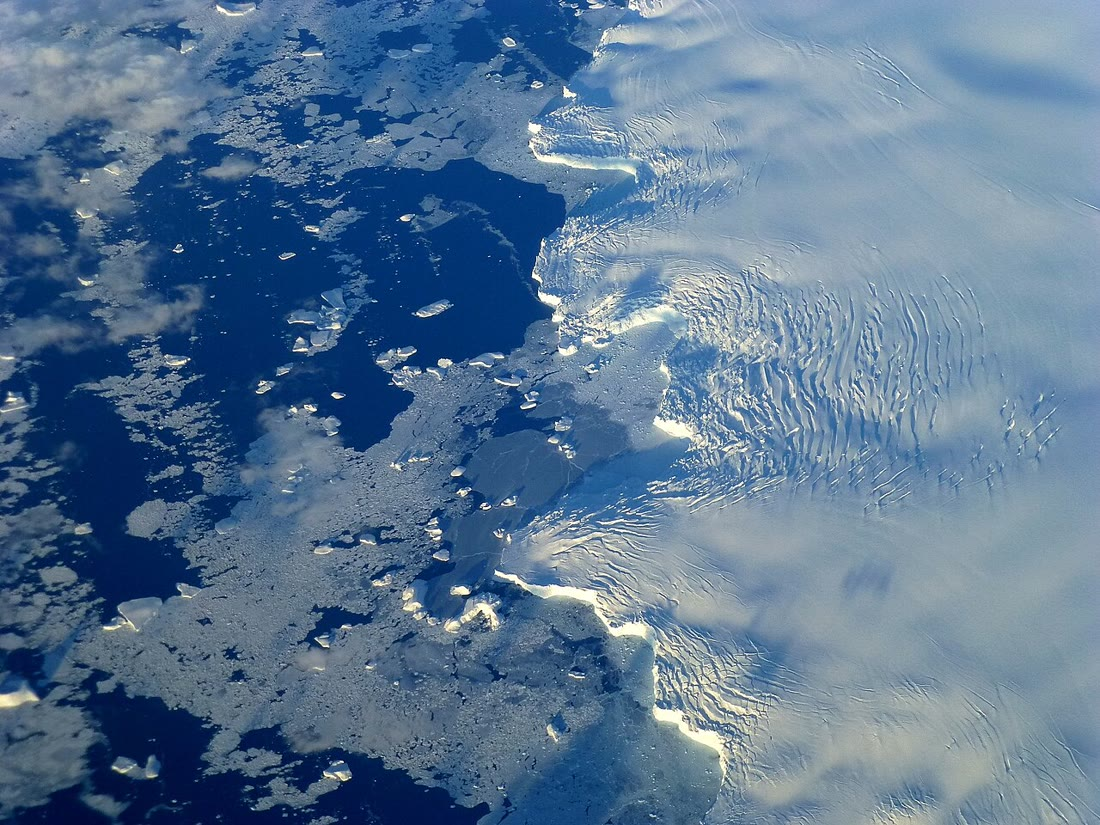
\includegraphics[width=\linewidth]{images/book1/g8-ice-shelf-edge.jpg}
\end{minipage}\hfill
\begin{minipage}[c]{0.46\linewidth}\raggedright
{\small \omterm{def:g3:continents-and-oceans:poles}{南极}半岛外阿德莱德岛附近\omterm{def:g8:ice-on-earth:ice-sheet}{冰架}的边缘，
由飞机于 2012 年 10 月 28~日拍摄。图右侧厚实、起皱的
白色冰体即为\omterm{def:g8:ice-on-earth:ice-sheet}{冰架}；左侧深色海水上漂着断裂的较薄
\omterm{def:g8:ice-on-earth:sea-ice}{海冰}块。NASA，Operation IceBridge
（公有领域，经由维基共享资源）。}
\end{minipage}
% ledger: commons:ice-shelf
\label{fig:g8:ice-on-earth:ice-shelf}
\end{omfigure}

\omterm{def:g8:ice-on-earth:ice-sheet}{冰盖}中所储存的水来自\omterm{def:g2:water-on-earth:ocean}{海洋}：海水蒸发，
以雪的形式降落并堆积于陆地上。若格陵兰岛的冰全部融化，
\omterm{def:g4:world-physical-map:altitude}{海平面}将上升约 \qty{7.4}{m}；若\omterm{def:g3:continents-and-oceans:poles}{南极}洲的冰全部融化，
则上升约 \qty{58}{m}。全球所有山地\omterm{def:g8:ice-on-earth:glacier}{冰川}，数量超过
\num{200000} 条，合计会使\omterm{def:g4:world-physical-map:altitude}{海平面}上升不足半米。
% ledger: nsidc:ice-sheets, nsidc:ice-cover

\begin{omfigure}
\begin{tikzpicture}
\begin{axis}[omrecord, xbar, width=10.5cm, height=3.6cm, xmin=0, xmax=68,
  bar width=9pt, ytick=data, symbolic y coords={glaciers,Greenland,Antarctica},
  yticklabels={所有山地冰川, 格陵兰冰盖, 南极冰盖},
  xlabel={全部融化后海平面上升（m）}, enlarge y limits=0.3,
  nodes near coords, nodes near coords style={font=\footnotesize, anchor=west, fill=white, inner sep=1.5pt},
  ymajorgrids=false]
  \addplot[fill=omIce!80!black, draw=black!60] coordinates {(0.5,glaciers) (7.4,Greenland) (58,Antarctica)};
\end{axis}
\end{tikzpicture}

{\small 各类陆地冰若完全融化，\omterm{def:g4:world-physical-map:altitude}{海平面}将上升多少，
（数值来自美国国家冰雪数据中心；\omterm{def:g8:ice-on-earth:glacier}{冰川}一项为上限，
“略低于半米”）。}
% ledger: nsidc:ice-sheets, nsidc:ice-cover
\label{fig:g8:ice-on-earth:sea-level-bars}
\end{omfigure}

漂浮的冰则不同。\omterm{def:g8:ice-on-earth:ice-sheet}{冰架}或\omterm{def:g8:ice-on-earth:ice-sheet}{冰山}本已浮于
海面之上：它已排开了与自身重量相等的海水。当它
破碎或融化时，\omterm{def:g4:world-physical-map:altitude}{海平面}不会上升。但\omterm{def:g8:ice-on-earth:ice-sheet}{冰架}会阻挡其后方的
\omterm{def:g8:ice-on-earth:glacier}{冰川}，好比瓶塞；\omterm{def:g3:continents-and-oceans:poles}{南极}洲的拉尔森 B \omterm{def:g8:ice-on-earth:ice-sheet}{冰架}
于 2002 年崩裂后，其后方的\omterm{def:g8:ice-on-earth:glacier}{冰川}加速，
部分\omterm{def:g8:ice-on-earth:glacier}{冰川}的速度达到原来的八倍，并将更多陆地冰注入
\omterm{def:g2:water-on-earth:ocean}{海洋}。
% ledger: nsidc:ice-shelves

\begin{inthelab}[漂浮的冰与陆地上的冰]
在室内，向两只透明玻璃杯中各放入一块小石子，使其
加水后露出水面。在第一只杯中，让几块冰块
漂浮在水面上。在第二只杯中，将相同数量的冰块
架在石子上，置于水面以上。两只杯中都加水至
同一水位，并用记号笔做标记。待所有冰块
全部融化后，比较水位与标记。哪只杯子的情况
表现与\omterm{def:g8:ice-on-earth:ice-sheet}{冰山}融化时的\omterm{def:g4:world-physical-map:altitude}{海平面}一致，哪只杯子
表现与\omterm{def:g8:ice-on-earth:ice-sheet}{冰盖}融化时的\omterm{def:g4:world-physical-map:altitude}{海平面}一致？
\end{inthelab}

\section{海冰}

\omterm{def:g8:ice-on-earth:sea-ice}{海冰}则是另一回事：它本身就是冻结的海水。每
年冬季，极地\omterm{def:g2:water-on-earth:ocean}{海洋}表面都大面积冻结；每
年夏季，大部分\omterm{def:g8:ice-on-earth:sea-ice}{海冰}又会融化。在\omterm{def:g3:continents-and-oceans:poles}{北极}，\omterm{def:g8:ice-on-earth:sea-ice}{海冰}面积
在夏末的 9 月最小，在冬末的 3 月最大。
卫星已测量其\emph{\omterm{def:g8:ice-on-earth:sea-ice}{海冰}范围}，即海面上
冰覆盖率至少为 15~\% 的区域面积，
自 20 世纪 70 年代末起每日测得。
% ledger: nsidc:sea-ice-def

\begin{definition}[海冰]\label{def:g8:ice-on-earth:sea-ice}
\emph{海冰}\index{海冰}是冻结的海水：它在\omterm{def:g2:water-on-earth:ocean}{海洋}中
直接形成、生长并融化。它不同于\omterm{def:g8:ice-on-earth:ice-sheet}{冰山}与\omterm{def:g8:ice-on-earth:ice-sheet}{冰架}，
后两者虽漂浮于海面上，却由陆地上降落的雪形成。
\end{definition}
% ledger: nsidc:sea-ice-def

\omterm{def:g8:ice-on-earth:sea-ice}{海冰}的影响远不止于极地。开阔的海水颜色深暗：它反射
照射到其上的阳光仅约 6~\%，其余则被吸收。\omterm{def:g8:ice-on-earth:sea-ice}{海冰}
反射 50 至 70~\%，覆有积雪的\omterm{def:g8:ice-on-earth:sea-ice}{海冰}可反射高达 90~\%。当
\omterm{def:g8:ice-on-earth:sea-ice}{海冰}融化时，下方深色的海水吸收更多的太阳
能量而升温，从而使更多\omterm{def:g8:ice-on-earth:sea-ice}{海冰}融化。
% ledger: nsidc:sea-ice-reflect

\begin{omfigure}
\begin{tikzpicture}
\begin{axis}[omrecord, width=13cm, height=5.4cm, xmin=1977, xmax=2027,
  ymin=3, ymax=8.2, xtick={1980,1990,...,2020},
  x tick label style={/pgf/number format/1000 sep={}},
  xlabel={年}, ylabel={范围（百万 km$^2$）},
  legend style={at={(0.98,0.97)}, anchor=north east, draw=none, fill=white}]
  \addplot[omCold, mark=*, mark size=1.3pt, line width=0.6pt]
    table[x=year, y=extent_Mkm2] {figdata/out/grade-8-sea_ice-extent.dat};
  \addlegendentry{九月平均范围}
  \addplot[omWarm, dashed, line width=1pt]
    table[x=year, y=extent_Mkm2] {figdata/out/grade-8-sea_ice-trend.dat};
  \addlegendentry{趋势线}
  \node[font=\scriptsize, anchor=north] at (axis cs:2012,3.5) {2012};
\end{axis}
\end{tikzpicture}

{\small \omterm{def:g3:continents-and-oceans:poles}{北极}\omterm{def:g8:ice-on-earth:sea-ice}{海冰}每年 9 月的范围，1979--2025 年，以及
最能拟合各数据点的直线。数据来自 NSIDC Sea Ice Index，
第~4~版（F.~Fetterer 等，2025）。}
% ledger: data:b1-nsidc-sea-ice (figdata/grade-8/sea_ice.py)
\label{fig:g8:ice-on-earth:sea-ice}
\end{omfigure}

各数据点逐年有起有伏：每个夏天的\omterm{def:g1:watching-the-weather:weather}{天气}都会影响数值。
但多年来，数据明显在下降。为了看清起伏之下的变化，
科学家画出\emph{趋势线}，
即尽可能靠近所有数据点的直线。
% ledger: data:b1-nsidc-sea-ice (figdata/grade-8/sea_ice.py)

\begin{method}[读懂图中的趋势]
\begin{enumerate}
  \item 读懂坐标轴：测量的是什么、用什么单位、跨越哪些年份。
  \item 观察数据点：起伏背后，总体是上升、下降，
        还是基本不变？
  \item 分别读出趋势线在第一年和最后一年的数值。
  \item 求两者之差，再除以两者之间的年数
        （或十年数）：这就是每年
        （或每十年）的平均变化量。
  \item 不要对某一年过度解读：
        偏离直线很远的单个点反映的是\omterm{def:g1:watching-the-weather:weather}{天气}，直线才代表趋势。
\end{enumerate}
\end{method}

\begin{example}[北极九月的海冰]
由图可见，1979 年趋势线约为 760 万~\unit{km^2}，
2025 年约为 410 万~\unit{km^2}。变化量为 $7.6 - 4.1 =
3.5$ 百万~km$^2$，历时 $2025 - 1979 = 46$ 年，即 4.6 个十年：
$3.5 \div 4.6 \approx 0.76$。九月\omterm{def:g8:ice-on-earth:sea-ice}{海冰}面积大约每十年减少
76 万~\unit{km^2}：46 年间，趋势线
几乎失去了 1979 年数值的一半。
2012 年的最低点 357 万~\unit{km^2} 远低于趋势线：
那年夏天是一个异常的年份。
\end{example}
% ledger: data:b1-nsidc-sea-ice (figdata/grade-8/sea_ice.py), nsidc:sea-ice-reflect

测量结果表明，随着\omterm{def:g3:continents-and-oceans:poles}{北极}变暖，
自 1980 年代以来，\omterm{def:g3:continents-and-oceans:poles}{北极}夏季\omterm{def:g8:ice-on-earth:sea-ice}{海冰}变得既更小又更薄。
\Cref{ch:g9:climate-past-and-present} 讨论地球\omterm{def:g5:weather-and-climate:climate}{气候}
如何变化，以及为何变化。
% ledger: nsidc:sea-ice-reflect

\section{永久冻土}

在遥远的北方，寒冷深入地下。
北美洲、格陵兰和北亚的苔原之下，土壤和\omterm{def:g3:stones-pebbles-sand:rock}{岩石}全年冻结，
许多地方已冻结数千年。
只有一层薄薄的表层，即\emph{活动层}，
每年夏季融化，冬季再次冻结；植物在其中生长，
而无法渗入下方冻土的水，
则在地表积成水洼。
% ledger: nsidc:permafrost

\begin{definition}[永久冻土]\label{def:g8:ice-on-earth:permafrost}
\emph{永久冻土}\index{永久冻土}是指地面、土壤或\omterm{def:g3:stones-pebbles-sand:rock}{岩石}，
其温度至少连续两年保持在 \qty{0}{\degreeCelsius} 或以下。
\end{definition}
% ledger: nsidc:permafrost

\omterm{def:g8:ice-on-earth:permafrost}{永久冻土}分布在约 2300 万~\unit{km^2} 的范围之下，约占\omterm{def:g3:continents-and-oceans:equator}{北半球}陆地的四分之一，
并位于阿拉斯加约 85~\% 的地区之下。充满冰的冻土坚硬如\omterm{def:g3:stones-pebbles-sand:rock}{岩石}；
冰融化后，地面变成泥浆并下陷。
道路开裂，建筑倾斜，管道可能破裂：
穿越\omterm{def:g8:ice-on-earth:permafrost}{永久冻土}区的阿拉斯加输油管道，有
\qty{676}{km} 架设在地面之上。\omterm{def:g8:ice-on-earth:permafrost}{永久冻土}融化还会使
其中冻结了数千年的植物遗体腐烂，
并向大气中释放二氧化碳和甲烷。
% ledger: nsidc:permafrost, nsidc:permafrost-thaw

\begin{omfigure}
\begin{minipage}[c]{0.5\linewidth}\centering
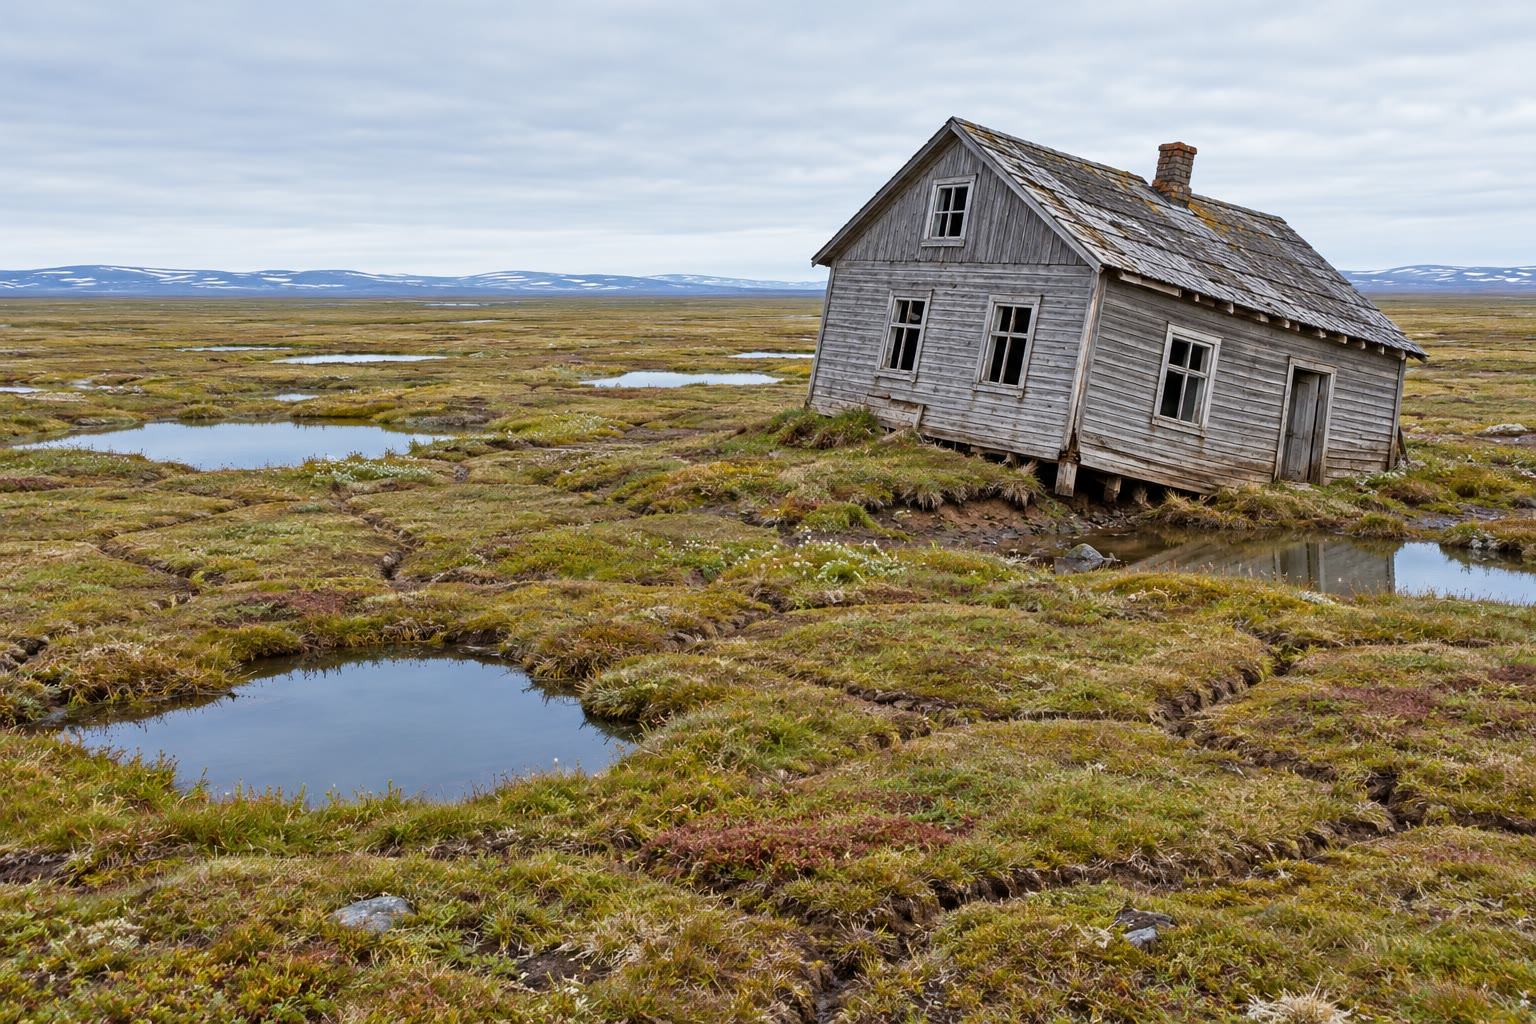
\includegraphics[width=\linewidth]{images/book1/ai/g8-permafrost-house.jpg}
\end{minipage}\hfill
\begin{minipage}[c]{0.46\linewidth}\centering
\begin{tikzpicture}[font=\footnotesize]
  \fill[omLithAlluv] (0,0) rectangle (3.2,-0.6);
  \fill[omIce!70!omLithShale] (0,-0.6) rectangle (3.2,-3.0);
  \foreach \x/\y in {0.4/-1.0, 1.5/-1.3, 2.6/-0.9, 0.9/-1.9, 2.1/-2.2, 0.5/-2.6, 2.8/-2.6}
    \fill[white] (\x,\y) ellipse (0.22 and 0.06);
  \fill[omLithShale!60] (0,-3.0) rectangle (3.2,-3.6);
  \draw[green!45!black, line width=1pt] (0,0) -- (3.2,0);
  \node[anchor=west, align=left] at (3.3,-0.3) {活动层：\\ 每年夏季 \\ 融化};
  \node[anchor=west, align=left] at (3.3,-1.8) {永久冻土：\\ 全年冻结，\\ 含冰透镜体};
  \node[anchor=west, align=left] at (3.3,-3.3) {未冻结 \\ 地层};
\end{tikzpicture}
\end{minipage}

\smallskip
{\small 左图：苔原上一座因\omterm{def:g8:ice-on-earth:permafrost}{永久冻土}融化而倾斜的房屋
（AI 生成的通用场景示意插图）。右图：
苔原之下的\omterm{def:g7:sediments-and-fossils:layer}{地层}（示意图，不按比例）。}
\label{fig:g8:ice-on-earth:permafrost}
\end{omfigure}

\section{冰期}

地球上的冰并非始终覆盖同一区域。大约 \num{20000}
年前，\omterm{def:g8:ice-on-earth:ice-sheet}{冰盖}覆盖了北美洲和北欧的大部分地区，
包括斯堪的纳维亚半岛。
那时\omterm{def:g8:ice-on-earth:glacier}{冰川}覆盖了约四分之一的陆地，而今天约为十分之一。
这些冰锁住了大量水，使\omterm{def:g4:world-physical-map:altitude}{海平面}
比今天低了 \qty{120}{m} 以上：今天\omterm{def:g8:the-oceans:seafloor}{大陆架}的部分区域曾是陆地。
大约 \num{15000} 年前，\omterm{def:g8:ice-on-earth:ice-sheet}{冰盖}开始融退，
\omterm{def:g4:world-physical-map:altitude}{海平面}随之上升；约 \num{8000} 年前，
\omterm{def:g4:world-physical-map:altitude}{海平面}已大致达到现在的高度。
% ledger: usgs:lgm, nsidc:ice-sheets, nsidc:ice-cover

\begin{definition}[冰期]\label{def:g8:ice-on-earth:ice-age}
\emph{冰期}\index{冰期}是地球历史上一段漫长的寒冷时期，\omterm{def:g8:ice-on-earth:ice-sheet}{冰盖}在此期间
向极地地区以外大范围扩展，覆盖\omterm{def:g3:continents-and-oceans:continent}{大陆}的大片区域。
最近一次冰期在约 \num{20000} 年前最为寒冷，
并于约 \num{12000} 年前结束。
\end{definition}
% ledger: usgs:lgm, nps:u-valley

末次\omterm{def:g8:ice-on-earth:ice-age}{冰期}的痕迹遍布它曾覆盖的陆地：
今天远离任何\omterm{def:g8:ice-on-earth:glacier}{冰川}的 \omterm{def:g8:ice-on-earth:glacial-landforms}{U 形谷}、横跨\omterm{def:g1:landscapes-around-us:landform}{平原}的终碛、
散落在田野上的漂砾。但它并非唯一的一次。
在过去几十万年间，\omterm{def:g8:ice-on-earth:ice-age}{冰期}与其间的温暖时期
反复交替；我们生活在一个温暖时期。
\Cref{ch:g9:climate-past-and-present}讲述了科学家
如何从\omterm{def:g3:continents-and-oceans:poles}{南极}冰层本身读取这段漫长的历史。
% ledger: nps:u-valley, nps:moraines, usgs:erratic

\section{练习}

\begin{exercise}[$\star$]\label{exo:g8:ice-on-earth:1}
利用本章中的\omterm{def:g8:ice-on-earth:glacier}{冰川}纵剖面图，指出：(a) \omterm{def:g8:ice-on-earth:glacier}{冰川}获得冰量的部分；
(b) \omterm{def:g8:ice-on-earth:glacier}{冰川}失去冰量的部分；(c) \omterm{def:g8:ice-on-earth:glacier}{冰川}的前缘；
(d) \omterm{def:g8:ice-on-earth:glacier}{冰川}末端的\omterm{def:g8:ice-on-earth:glacial-landforms}{冰碛}垄。
\end{exercise}

\begin{exercise}[$\star$]\label{exo:g8:ice-on-earth:2}
% ledger: nsidc:firn, nsidc:glacier-flow, nsidc:sea-ice-def
判断下列说法是否正确，并改正错误的句子：(a) \omterm{def:g8:ice-on-earth:glacier}{冰川}由
冻结的海水构成；(b) 雪大约需要一年才能变成粒雪；(c) \omterm{def:g8:ice-on-earth:glacier}{冰川}退缩时，
其冰向山上流动；(d) \omterm{def:g3:continents-and-oceans:poles}{北极}\omterm{def:g8:ice-on-earth:sea-ice}{海冰}的
范围在 9 月最小。
\end{exercise}

\begin{exercise}[$\star$]\label{exo:g8:ice-on-earth:3}
% ledger: usgs:erratic, nsidc:permafrost
给出下列描述对应的术语：(a) 谷底宽阔、谷坡陡峭、由\omterm{def:g8:ice-on-earth:glacier}{冰川}\omterm{def:g5:water-shapes-the-land:erosion}{侵蚀}形成的\omterm{def:g1:landscapes-around-us:landform}{山谷}；
(b) 被\omterm{def:g8:ice-on-earth:glacier}{冰川}从远处搬运而来的巨石；
(c) 仍与陆地冰相连的漂浮冰板；
(d) 至少连续两年保持冻结的地面。
\end{exercise}

\begin{exercise}[$\star$]\label{exo:g8:ice-on-earth:4}
% ledger: nsidc:ice-sheets, nsidc:ice-cover
(a) 今天哪两块陆地被\omterm{def:g8:ice-on-earth:ice-sheet}{冰盖}覆盖？
(b) 两者中哪一块的冰若全部融化，\omterm{def:g4:world-physical-map:altitude}{海平面}会上升更多？上升多少？
(c) 今天地球陆地中有多大比例被冰覆盖？
\end{exercise}

\begin{exercise}[$\star\star$]\label{exo:g8:ice-on-earth:5}
% ledger: data:b1-nsidc-sea-ice (figdata/grade-8/sea_ice.py)
利用 9 月\omterm{def:g3:continents-and-oceans:poles}{北极}\omterm{def:g8:ice-on-earth:sea-ice}{海冰}的图，(a) 读出 1979 年和 2012 年的范围；
(b) 这两年间减少了多少百万~km$^2$？
(c) 2012 年时，1979 年的范围减少了多大比例？
结果用简单分数表示。
(d) 为什么比较趋势线比比较两个单独年份更可靠？
\end{exercise}

\begin{exercise}[$\star\star$]\label{exo:g8:ice-on-earth:6}
% ledger: nsidc:muir, uw:pedersen
缪尔\omterm{def:g8:ice-on-earth:glacier}{冰川}的冰舌在 1941 年至 2004 年间后退了 \qty{12}{km}。(a) 这段时间有多少年？
(b) 其每年的平均退缩量是多少米？四舍五入到最近的十米。
(c) 佩德森\omterm{def:g8:ice-on-earth:glacier}{冰川}在 1984 年至 2021 年间后退了 \qty{3.2}{km}，
其每年的平均退缩量是多少？
(d) 哪条\omterm{def:g8:ice-on-earth:glacier}{冰川}后退得更快？
\end{exercise}

\begin{exercise}[$\star\star$]\label{exo:g8:ice-on-earth:7}
用几句话，按顺序说明高山上降落的雪
如何变成远在\omterm{def:g1:landscapes-around-us:landform}{山谷}下游的\omterm{def:g8:ice-on-earth:glacier}{冰川}冰舌处的冰。请使用
\emph{粒雪}、\emph{积累区}、\emph{流动}和
\emph{消融区}等词。
\end{exercise}

\begin{exercise}[$\star\star$]\label{exo:g8:ice-on-earth:8}
% ledger: nsidc:ice-shelves
两只玻璃杯注入相同高度的水。在杯 A 中，冰块漂浮在水面上；
在杯 B 中，同样的冰块放在水面上方的一块石头上。
(a) 冰融化后，哪只杯中的水位上升了？(b) 哪只杯是海中\omterm{def:g8:ice-on-earth:ice-sheet}{冰山}融化的模型？
哪只杯是陆地上\omterm{def:g8:ice-on-earth:ice-sheet}{冰盖}融化的模型？
(c) \omterm{def:g8:ice-on-earth:ice-sheet}{冰架}崩裂为什么仍
会影响\omterm{def:g4:world-physical-map:altitude}{海平面}的高低？
\end{exercise}

\begin{exercise}[$\star\star$]\label{exo:g8:ice-on-earth:9}
一位徒步者穿越一条宽阔的\omterm{def:g1:landscapes-around-us:landform}{山谷}，谷底平坦，谷坡非常陡峭。在
一片田野中央，她发现一块与汽车一样大的花岗岩巨石；\omterm{def:g1:landscapes-around-us:landform}{山谷}中的\omterm{def:g3:stones-pebbles-sand:rock}{岩石}全部是石灰岩。
在较高处，一道由杂乱石块组成的长长的岩堆沿着谷坡延伸。
(a) \omterm{def:g1:landscapes-around-us:landform}{山谷}是什么形状？是什么\omterm{def:g5:water-shapes-the-land:erosion}{侵蚀}形成的？
(b) 巨石是怎样到达那里的？它叫什么？
(c) 这道岩堆是什么？它在谷坡上的高度说明了什么？
\end{exercise}

\begin{exercise}[$\star\star$]\label{exo:g8:ice-on-earth:10}
% ledger: nsidc:ice-sheets
若\omterm{def:g3:continents-and-oceans:poles}{南极}\omterm{def:g8:ice-on-earth:ice-sheet}{冰盖}全部融化，\omterm{def:g4:world-physical-map:altitude}{海平面}将上升约 \qty{58}{m}；若格陵兰\omterm{def:g8:ice-on-earth:ice-sheet}{冰盖}全部融化，\omterm{def:g4:world-physical-map:altitude}{海平面}将上升约
\qty{7.4}{m}。(a) 格陵兰冰量的十分之一会使\omterm{def:g4:world-physical-map:altitude}{海平面}上升多少？
(b) \omterm{def:g3:continents-and-oceans:poles}{南极}冰量的百分之一会使\omterm{def:g4:world-physical-map:altitude}{海平面}上升多少？
(c) \omterm{def:g3:continents-and-oceans:poles}{南极}所含的冰量是格陵兰的多少倍？
四舍五入为最接近的整数。
\end{exercise}

\begin{exercise}[$\star\star\star$]\label{exo:g8:ice-on-earth:11}
% ledger: data:b1-nsidc-sea-ice (figdata/grade-8/sea_ice.py: mean_1980s, mean_2010s, trend)
9 月\omterm{def:g3:continents-and-oceans:poles}{北极}\omterm{def:g8:ice-on-earth:sea-ice}{海冰}的平均范围在
1980--1989 年间为 721 万~\unit{km^2}，
2010--2019 年间为 465 万~\unit{km^2}。(a) 一百万即
$10^6$。将两个数值都写成 km$^2$，不要用“百万”一词。
(b) 这两个十年间，平均范围减少了多少？
(c) 这两个十年相隔 30 年。
平均每十年减少多少？将其与趋势线给出的
每十年 76 万~\unit{km^2} 进行比较。
(d) 为什么直线趋势线不能无限延伸到未来？
\end{exercise}

\begin{exercise}[$\star\star\star$]\label{exo:g8:ice-on-earth:12}
% ledger: usgs:lgm (the shelf slope is exercise data)
约 \num{20000} 年前，\omterm{def:g4:world-physical-map:altitude}{海平面}比今天低约 \qty{120}{m}。在
某\omterm{def:g1:landscapes-around-us:water}{海岸}外，\omterm{def:g8:the-oceans:seafloor}{大陆架}向海缓慢倾斜，每向外海延伸 \qty{1}{km}，下降 \qty{1}{m}（练习数据）。
(a) 当时的\omterm{def:g1:landscapes-around-us:water}{海岸}线位于向外海多远处？
(b) \omterm{def:g4:world-physical-map:altitude}{海平面}下降所缺失的 \qty{120}{m} 海水去了哪里？
(c) 解释为什么今天在远离任何\omterm{def:g4:world-physical-map:range}{山脉}的
\omterm{def:g1:landscapes-around-us:landform}{平原}上发现的终碛，是同一次\omterm{def:g8:ice-on-earth:ice-age}{冰期}的证据。
\end{exercise}

\section{问题：冰川的长期退缩}

\begin{problem}[{周末问题——一条山地冰川的前缘
自 1960 年起每十年测量一次，计算其退缩速度，
并读出它留下的山谷}]
\label{pb:g8:ice-on-earth:1}
% ledger: nsidc:muir, uw:pedersen, nps:moraines (figdata/grade-8/glacier_retreat.py; Glacier G and its measurements are exercise data)
自 1960 年起，每十年一次，一支考察队测量了
\omterm{def:g8:ice-on-earth:glacier}{冰川}~G 冰舌的位置。\omterm{def:g8:ice-on-earth:glacier}{冰川}~G 是山中的\omterm{def:g1:landscapes-around-us:landform}{山谷}\omterm{def:g8:ice-on-earth:glacier}{冰川}，其距离
自\omterm{def:g3:stones-pebbles-sand:rock}{岩石}标志~R 沿\omterm{def:g1:landscapes-around-us:landform}{山谷}向上量取。R 于 1960 年冰舌处
涂在谷底上。小屋~H 紧靠谷底，位于 R 沿\omterm{def:g1:landscapes-around-us:landform}{山谷}向上
\qty{1980}{m} 处。图中标出各次测量时的冰舌位置，
以及 1960 年冰舌下方的山脊。

\begin{center}
\begin{tikzpicture}
\begin{axis}[axis equal image, width=12.5cm, xmin=-500, xmax=2600, ymin=-760, ymax=760,
  axis lines=none, clip=true]
  \fill[black!13] (axis cs:-500,-760) rectangle (axis cs:2600,760);
  \addplot[fill=white, draw=none] table[x=y, y=x] {figdata/out/grade-8-glacier_retreat-floor.dat} -- cycle;
  \addplot[fill=omIce, draw=none] table[x=y, y=x] {figdata/out/grade-8-glacier_retreat-ice.dat} -- cycle;
  \addplot[black!70, line width=0.8pt] table[x=y, y=x] {figdata/out/grade-8-glacier_retreat-walls.dat};
  \addplot[omCold, line width=0.9pt] table[x=y, y=x] {figdata/out/grade-8-glacier_retreat-fronts.dat};
  \addplot[omLithCongl!80!black, line width=3pt] table[x=y, y=x] {figdata/out/grade-8-glacier_retreat-moraine.dat};
  \addplot[only marks, mark=none, nodes near coords, point meta=explicit symbolic,
    every node near coord/.style={anchor=south, rotate=90, font=\scriptsize, inner sep=1pt}]
    table[x=y, y=x, meta=year] {figdata/out/grade-8-glacier_retreat-labels.dat};
  \addplot[only marks, mark=*, mark size=2pt] coordinates {(0,0)};
  \node[font=\footnotesize\bfseries, anchor=south east] at (axis cs:-10,10) {R};
  \addplot[only marks, mark=square*, mark size=2.6pt, omDef] coordinates {(1980,-560)};
  \node[font=\footnotesize\bfseries, anchor=north] at (axis cs:1980,-590) {H};
  \node[font=\scriptsize, anchor=west] at (axis cs:-480,-590) {沿山谷向上 $\longrightarrow$};
  \node[font=\scriptsize] at (axis cs:2250,0) {2020 年的冰};
  \draw[black, line width=1.2pt] (axis cs:2000,640) -- (axis cs:2500,640)
    node[midway, below, font=\scriptsize] {\qty{500}{m}};
\end{axis}
\end{tikzpicture}

\smallskip
{\small
\begin{tabular}{|l|c|c|c|c|c|c|c|}
\hline
年份 & 1960 & 1970 & 1980 & 1990 & 2000 & 2010 & 2020 \\
\hline
冰舌距 R 的距离（m） & 0 & 180 & 330 & 520 & 700 & 880 & 1080 \\
\hline
\end{tabular}}
\end{center}

\noindent\textbf{第一部分——冰舌的位置。}\par\nopagebreak
\begin{enumerate}[beginpenalty=10000]
  \item 1960 年至 2020 年间，冰舌后退了多远？
  \item 计算每十年中冰舌后退的距离，
        其中哪个十年后退最少？哪个最多？
  \item \omterm{def:g8:ice-on-earth:glacier}{冰川}是否已停止顺坡流动？请说明理由。
  \item 1960 年冰舌正下方的暗色山脊由杂乱的\omterm{def:g3:stones-pebbles-sand:rock}{岩石}碎屑构成，
        它叫什么名称？它是如何形成的？
\end{enumerate}

\noindent\textbf{第二部分——退缩速度。}\par\nopagebreak
\begin{enumerate}[resume, beginpenalty=10000]
  \item 1960 年至 2020 年间，平均每十年退缩多少？
  \item 每年呢？
  \item 缪尔\omterm{def:g8:ice-on-earth:glacier}{冰川}在 63 年间后退了 \qty{12}{km}，
        平均每年约 \qty{190}{m}。这一速度是
        \omterm{def:g8:ice-on-earth:glacier}{冰川}~G 的多少倍？
  \item \omterm{def:g8:ice-on-earth:glacier}{冰川}~G 在积累区获得的冰量，比在消融区损失的
        冰量多还是少？请说明理由。
\end{enumerate}

\noindent\textbf{第三部分——它留下的\omterm{def:g1:landscapes-around-us:landform}{山谷}。}\par\nopagebreak
\begin{enumerate}[resume, beginpenalty=10000]
  \item 你认为 R 与 2020 年冰舌之间的谷底，
        其横截面应呈什么形状？为什么？
  \item 2020 年，冰舌距小屋所在高度有多远？
  \item 按第二部分的平均速度，冰舌需要多少年才能
        到达小屋所在的高度？那将是哪一年？
  \item 请给出一个理由，说明这一年并不是预测。
\end{enumerate}
\end{problem}
